\documentclass{article}
\usepackage{graphicx}

\begin{document}

\title{Homework Submission Servlet Teaching Assistant Documentation}
\author{Mike Burns}
\date{\today}

\maketitle

\section{Log-In Page}\label{sec:login}

\begin{figure}[h]
\centering
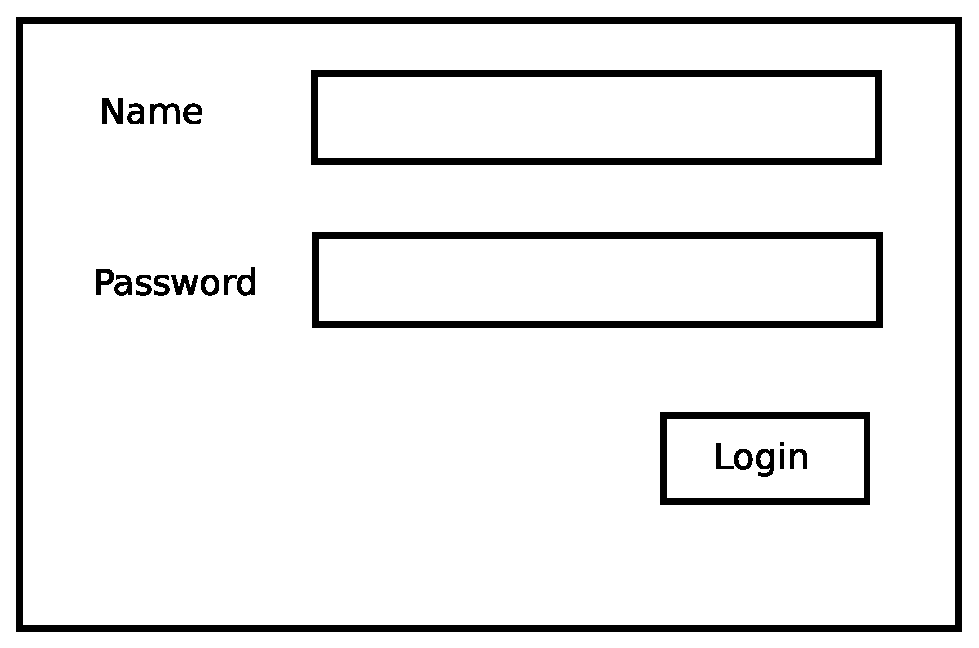
\includegraphics[scale=.35]{login.eps}
\caption{The Log-In Page}
\label{fig:login}
\end{figure}

Enter your username and password into the appropriate fields on the log-in
page.

\section{Logged-In Page}\label{sec:logged-in}

\begin{figure}[h]
\centering
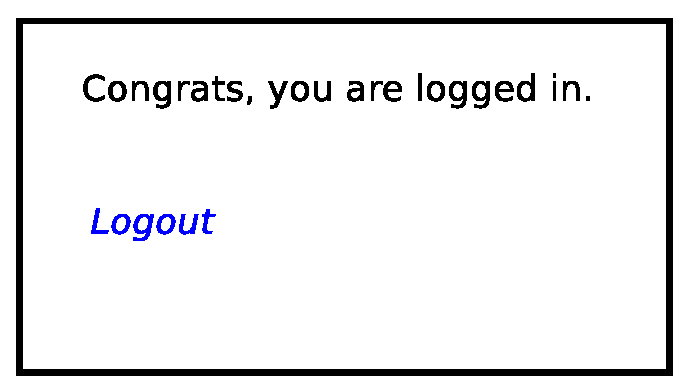
\includegraphics[scale=.35]{logged-in.eps}
\caption{The Logged-In Page}
\label{fig:logged-in}
\end{figure}

To log out, select the ``Logout'' hyperlink.

\section{Restarting The Web Server}

\begin{description}
\item[bin/stop-web-server]{Stop the Web server if it is running.}
\item[bin/start-web-server]{Start the Web server if it is not running.}
\end{description}

\section{Adding and Removing Users}

\begin{enumerate}
\item{Stop the Web server.}
\item{Edit the file \verb|etc/passwd|.}
\item{Start the Web server.}
\end{enumerate}

\end{document}
